% A Bloch sphere of radius |a| = 1 contains all possible states of a two-state quantum system (qubit).
% Each Bloch vector fully determines a spin-1/2 density matrix.
% Used in Exercise Sheet 10 of Statistical Physics by Manfred Salmhofer (2016), available at https://janosh.dev/physics/statistical-physics.

\documentclass{article}

\usepackage{tikz}

\usepackage{graphicx}
\usetikzlibrary{angles, quotes}
	\usetikzlibrary{arrows.meta, positioning, quotes, shapes, shapes.geometric}
\begin{document}


\definecolor{baseline6}{HTML}{6940FF}
\definecolor{baseline5}{HTML}{A12EFF}
\definecolor{baseline4}{HTML}{D24AFF}
\definecolor{baseline3}{HTML}{FF7DF0}
\definecolor{baseline2}{HTML}{FFBDD4}

\definecolor{thick6}{HTML}{00BDA8}
\definecolor{thick2}{HTML}{77F3DB}

\definecolor{thin6}{HTML}{D47E04}
\definecolor{thin2}{HTML}{FFDA09}

\definecolor{single}{HTML}{00A2FF}
\definecolor{full}{HTML}{425df5}

\definecolor{expt1col}{HTML}{FF0099}
\definecolor{expt3col}{HTML}{527319}
\definecolor{expt2col}{HTML}{0000FF}

\tikzset{
	expt1/.style={
		draw, circle, color=expt1col, line width=4, align=center, scale=2},
	expt2/.style={
		draw, circle, color=expt2col, line width=4,  align=center, scale=2},
	expt3/.style={
		draw, circle, color=expt3col, line width=4, align=center, scale=2},
		illus/.style={draw, rectangle}
}

\tikzset{nodes={font=\sffamily\bfseries}} 

\begin{figure}


	
	\begin{tikzpicture}
		
		\def\r{6}
		\draw (0,0) edge[-Stealth, line width=1] ["Backchannel", sloped, pos=.3] (-2*\r/5,  -2*\r/3) ;
		\draw (0,0) edge[-Stealth, line width=1] ["Group Size", pos=.9] (\r, 0) ;
		\draw (0,0) edge[-Stealth, line width=1] ["Group coherence", sloped, pos=.35] (0, \r);
		
		\node (n2) at (0,0) [expt1, fill=baseline2, label={[expt1col]below:2}] {};
		\node (n3) at (1,0) [expt1, fill=baseline3, label={[expt1col]below:3}]{};
		\node (n4) at (2,0) [expt1, fill=baseline4, label={[expt1col]below:4}] {};
		\node (n5) at (3,0) [expt1, fill=baseline5, label={[expt1col]below:5}] {};
		\node (n6) at (4,0) [expt1, fill=baseline6] {};
		\node[align=center,anchor=north,text=expt1col] at (4.6,-.45) {6 baseline};
		
		\node (n2thick) at (0,4) [expt3, fill=thick2, label= {[expt3col]above right:2 thick}] {};
		\node (n6thick) at (4,4) [expt3, fill=thick6, label={[expt3col]right:6 thick}] {};
		
		\node (nfull) at (4,1.5) [expt2, fill=full, label={[expt2col]right:6 full feedback}] {};
		\node (nsingle) at (4,3) [expt2, fill=single, label={[expt2col]right:6 single speaker}] {};
		
		\node (n2thin) at (-3/2,-5/2) [expt3, fill=thin2, label={[expt3col]below right: 2 thin}] {};
		\node (n6thin2) at (2.7,-2.3) [expt2, fill=thin6, label={[expt2col] right: 6 thin}] {};
		\node (n6thin) at (2.5,-2.5) [expt3, fill=thin6, label={[expt3col]below right: 6 thin}] {};
		
		\node[align=center,anchor=north] (lab1) at (-2,3) {Rotating speaker;\\limited feedback};
		\node[align=center,anchor=north] (lab2) at (-1.5,6) {Single speaker;\\full feedback};
		\node[align=center,anchor=north] (lab3) at (-3,0.2) {Listeners \\use chat};
		\node[align=center,anchor=north] (lab4) at (-3.5,-2.5) {Listeners \\use emoji};
		
		\node[align=center,anchor=north, text=expt1col] (ex1) at (2,1) {Experiment 1};
		\node[align=center,anchor=north, text=expt2col] (ex1) at (2,2.75) {Experiment 2};
		\node[align=center,anchor=north, text=expt3col] (ex1) at (.7,-1.7) {Experiment 3};
		
		
		\node[illus, anchor=north] () at (-3.5,-3.5) {	
\includegraphics[scale=.13]{images/nochat.png}};
		\node[illus, anchor=north] () at (-3.3,-.7) {
\includegraphics[scale=.13]{images/chat.png}};
			
		\node[illus, anchor=north] () at (-3.35,2) {
\includegraphics[scale=.08]{images/rotate.png}};
		\node[illus, anchor=north] () at (7.5,4.8) {
\includegraphics[scale=.08]{images/norotate.png}};
		
		
		\node[anchor=north] () at (-1,.7) {
\includegraphics[scale=.05]{images/two.png}};
		\node[ anchor=north] () at (6.8,.8) {
\includegraphics[scale=.05]{images/six.png}};
		
		\node[illus, anchor=north] () at (-4.3,4) {	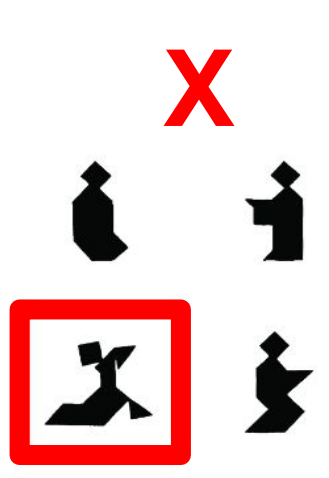
\includegraphics[scale=.1]{images/limited-wrong.png}	%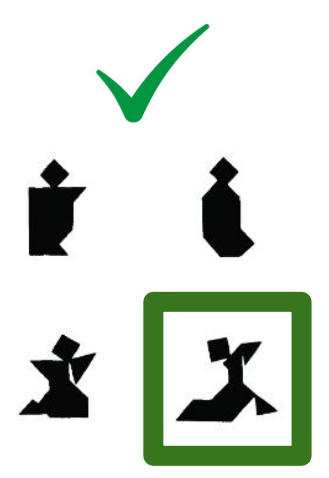
\includegraphics[scale=.1]{images/limited-correct.png}
		};
		\node[illus, anchor=north] () at (8,2.5) {	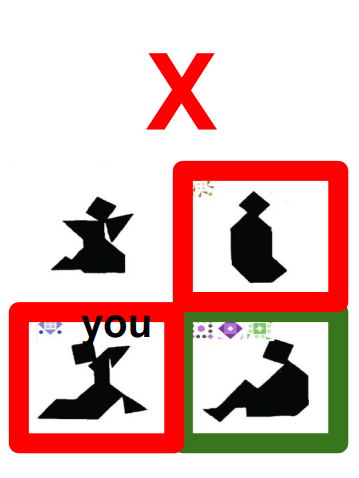
\includegraphics[scale=.1]{images/full-wrong.png}	%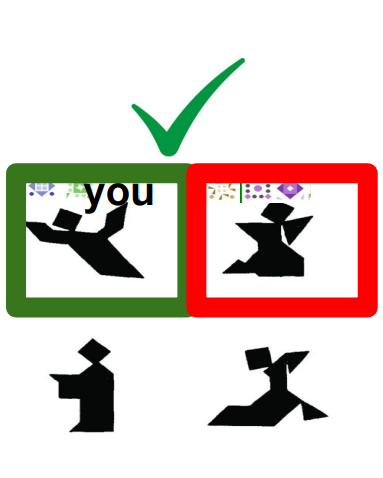
\includegraphics[scale=.1]{images/full-correct.png}
		};
		
		\draw[dashed] (n6) edge [] (n6thin);
		\draw[dashed] (n2thin) edge [] (n6thin);
		\draw[dashed] (n2thick) edge [] (n6thick);
		\draw[dashed] (n6) edge [] (n6thick);
		
		\begin{scope}[line width=1 pt, >=Stealth]
			\draw[->] (lab1) -> (n2);
			\draw[->] (lab2) -> (n2thick);
			\draw[->] (lab3) -> (n2);
			\draw[->] (lab4) -> (n2thin);
		\end{scope}
		
	\end{tikzpicture}
	
	\caption{ TODO }
	\label{diagram}
\end{figure}



	

\end{document}